\documentclass{article}
% Chinese
% \documentclass[UTF8, nofonts, mathptmx, 12pt, onecolumn]{article}
% \usepackage{xeCJK}
% \setCJKmainfont{SimSun}
\usepackage{amsmath}
\usepackage{amsfonts}
\usepackage{amssymb}
\usepackage{wasysym}
% \usepackage{ctex}
\usepackage{graphicx}
\usepackage{float}
\usepackage{geometry}
\geometry{a4paper,scale=0.8}
\usepackage{caption}
\usepackage{subcaption}
% \newcommand{\oiint}{\mathop{{\int\!\!\!\!\!\int}\mkern-21mu \bigcirc} {}}
\newcommand*{\dif}{\mathop{}\!\mathrm{d}}
\newcommand*{\md}{\mathop{}\!\mathrm{d}}
\newcommand*{\me}{\mathrm{e}}

% \usepackage{parskip}
% \setlength{\parindent}{0cm}

\usepackage{bm}
\let\Oldmathbf\mathbf
\renewcommand{\mathbf}[1]{\boldsymbol{\Oldmathbf{#1}}}
\let\eqnarray\align

\author{Xiping Hu}
\usepackage{authblk}
\author{Xiping Hu}
\affil{http://thehxp.tech/}
\title{Homework for Chapter 3}

\begin{document}
\maketitle

\begin{figure}[H]
  \centering
  
\includegraphics[width=\linewidth]{figures/Problem2-1}
  \label{fig:}
\end{figure}
\begin{figure}[H]
  \centering
  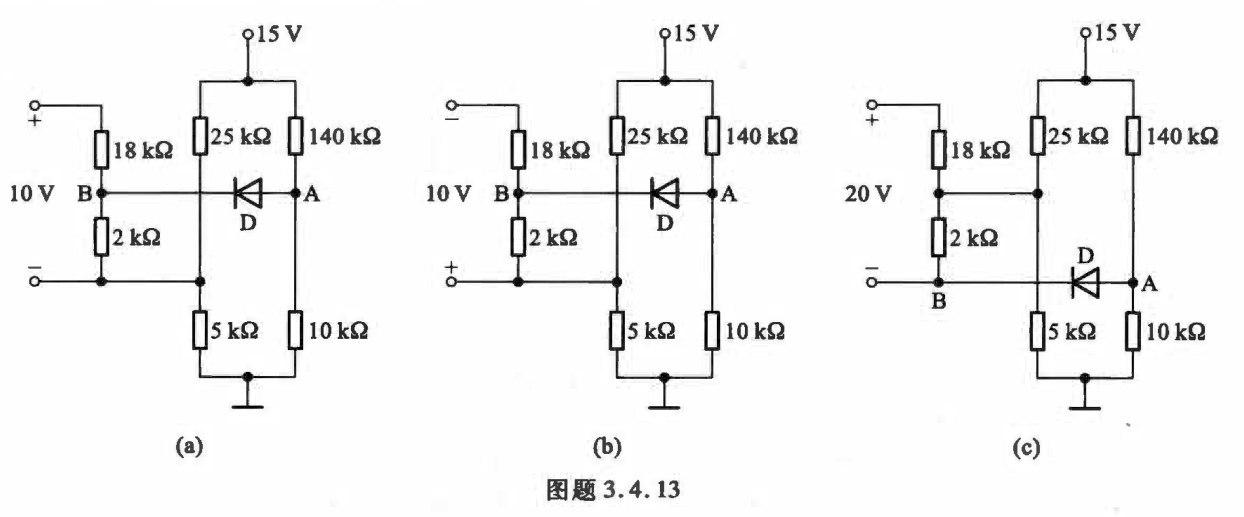
\includegraphics[width=0.7\linewidth]{figures/Problem2-2}
  \label{fig:}
\end{figure}

We first assume that the dipoles are all off

\begin{figure}[H]
  \centering
  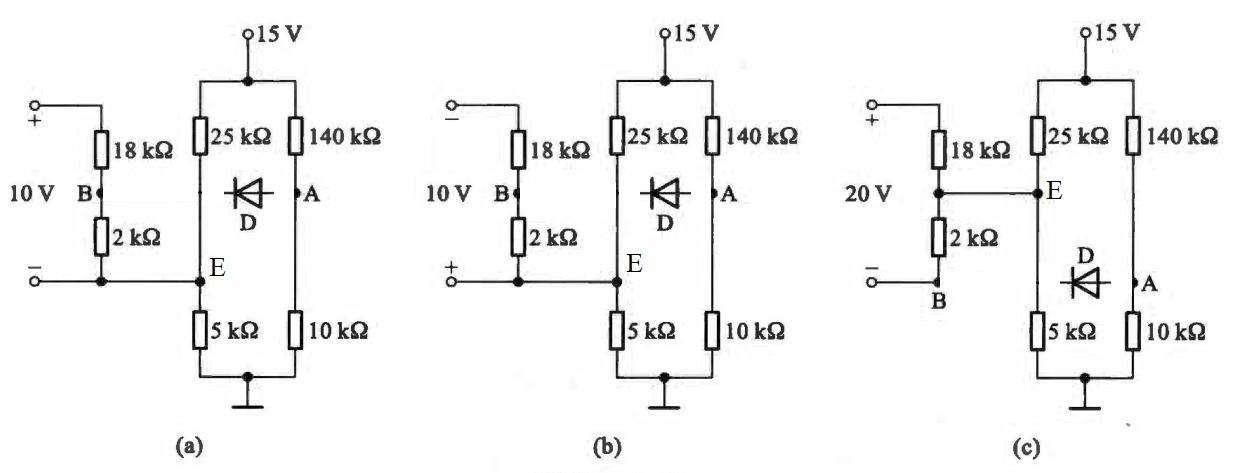
\includegraphics[width=0.7\linewidth]{figures/Problem2-3}
  \label{fig:}
\end{figure}

As for (a):

\begin{equation*}
  \begin{aligned}
    v_E &= \dfrac{5}{5 + 25} \times 15 = 2.5 \  \mathrm{V} \\
    v_A &= \dfrac{10}{10 + 140} \times 15 = 1 \  \mathrm{V} \\
    v_B &= \dfrac{2}{18 + 2} \times 10 + 2.5 = 3.5 \  \mathrm{V} 
  \end{aligned}
\end{equation*}

Since $v_B > v_A$, the dipole is off.

As for (b):

\begin{equation*}
  \begin{aligned}
    v_E &= \dfrac{5}{5 + 25} \times 15 = 2.5 \  \mathrm{V} \\
    v_A &= \dfrac{10}{10 + 140} \times 15 = 1 \  \mathrm{V} \\
    v_B &= - \dfrac{2}{18 + 2} \times 10 + 2.5 = 1.5 \  \mathrm{V} 
  \end{aligned}
\end{equation*}

Since $v_B > v_A$, the dipole is off.

As for (c):

\begin{equation*}
  \begin{aligned}
    v_E &= \dfrac{5}{5 + 25} \times 15 = 2.5 \  \mathrm{V} \\
    v_A &= \dfrac{10}{10 + 140} \times 15 = 1 \  \mathrm{V} \\
    v_B &= - \dfrac{2}{18 + 2} \times 20 + 2.5 = 0.5 \  \mathrm{V} 
  \end{aligned}
\end{equation*}

Since $v_B < v_A$, the dipole is on.


\end{document}